%%----------------------------------------------------------------------------
%% Presentatie HoGent Bedrijf en Organisatie
%%----------------------------------------------------------------------------
%% Auteur: Bert Van Vreckem [bert.vanvreckem@hogent.be]

\documentclass{beamer}

%==============================================================================
% Aanloop
%==============================================================================

%---------- Packages ----------------------------------------------------------

\usepackage{graphicx,multicol}
\usepackage{comment,enumerate,hyperref}
\usepackage{amsmath,amsfonts,amssymb}
\usepackage{tikz}
\usepackage[english]{babel}
\usepackage[utf8]{inputenc}
\usepackage{multirow}
\usepackage{eurosym}
\usepackage{listings}
\usepackage[T1]{fontenc}
\usepackage{lmodern}
\usepackage{textcomp}
\usepackage{framed}
\usepackage{wrapfig}

%---------- Configuratie ------------------------------------------------------

\usetikzlibrary{arrows,shapes,backgrounds,positioning,shadows}

\usetheme{hogent}

%---------- Commando-definities -----------------------------------------------

\newcommand{\tabitem}{~~\llap{\textbullet}~~}

%---------- Info over de presentatie ------------------------------------------

\title[Intro]{Research techniques\\1. The research process}
\author{Anita Bernard, Jens Buysse, Bert {Van Vreckem}}
\date{AY 2016-2017}

%==============================================================================
% Inhoud presentatie
%==============================================================================

\begin{document}

%---------- Front matter ------------------------------------------------------

% Dia met het HoGent logo
\HoGentLogo

% Titeldia met faculteitslogo
\titleframe

%---------- Inhoud ------------------------------------------------------------

\begin{frame}
  \frametitle{Contents}

  \tableofcontents
\end{frame}

\section{The scientific method}

\sectionframelogo{\normalsize{\emph{No matter how many instances of white swans we may have observed, this does not justify the conclusion that all swans are white}\\---Karl Popper}}

\begin{frame}
  \scaledimg{img/les1-01}
\end{frame}

\begin{frame}
  \frametitle{How do we gather knowledge?}

  \scaledimg{img/les1-02}
\end{frame}

\begin{frame}[plain,c]
  \begin{columns}
    \column{\dimexpr\paperwidth}
    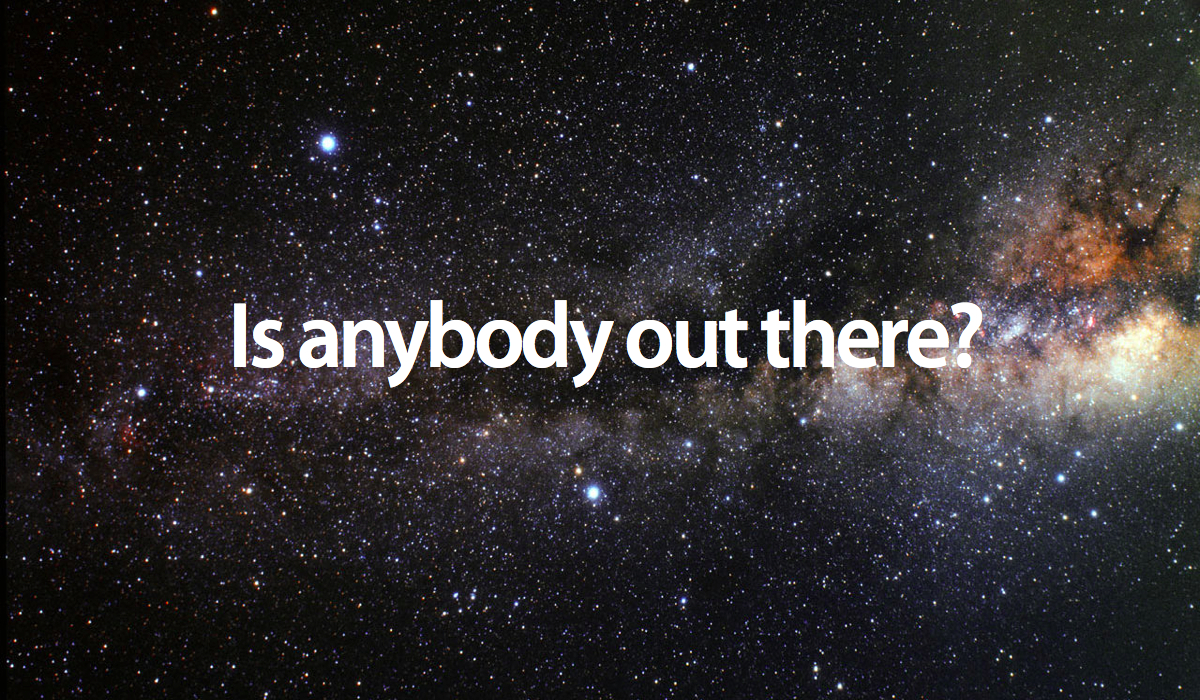
\includegraphics[width=\paperwidth]{img/les1-03}
  \end{columns}
\end{frame}

\begin{frame}
  \frametitle{How do we gather knowledge?}

  \begin{columns}[c]

  \column{.5\textwidth}
  Non-scientific method
    \begin{itemize}
    \item ``My gut feeling says it is''
    \item ``My father says so, so it should be true''
    \item ``There are many reports of UFO sightings, so there has to be something there''
    \item ``I read it on the Internet!''
    \end{itemize}

  \pause

  \column{.5\textwidth}
  Scientific method
    \begin{itemize}
    \item ``There are many planets''
    \item ``Molecules necessary for life are found everywhere''
    \item $\Rightarrow$ ``So it would surprise me if no life existed elsewhere in the universe''
    \item \textbf{But there is no proof as of yet}
    \end{itemize}

  \end{columns}
\end{frame}

\begin{frame}
  \frametitle{Can pigs fly?}
 % Bedoeling is hier de klas in 3 te delen: ene groep moet aantonen dat varkens kunnen vliegen op autoritaire wijze (bv. Bij boer Mcdonald gaan en navraag), de tweede op deductieve wijze (varkens zijn deel van gewervelden, sommige gewervelden hebben vleugels en dus .. (maar dus met verkeerde conclusie) en de derde tracht dit op wetenschappelijke methode. Hier kan voor deductie ook ik kan in pyama, pyama kan in koffer, dus ik kan in koffer gebruikt worden. 
  \scaledimg{img/les1-04}
\end{frame}

\begin{frame}
  \frametitle{The scientific method}

  Empirical research may have several goals:

  \begin{enumerate}
    \item Exploration
    \item Description
    \item Prediction
    \item Verification
  \end{enumerate}
\end{frame}

\begin{frame}
  \frametitle{The scientific method}

  \begin{columns}[c]

    \column{0.8\textwidth}
    \begin{itemize}
      \item Generalisation
        \begin{itemize}
          \item E.g. ``Agression is common in this part of the population''
        \end{itemize}
      \item Understanding
        \begin{itemize}
          \item There is a relation between frustration and agression
          \item Theory development
        \end{itemize}
    \end{itemize}

    \column{0.2\textwidth}
    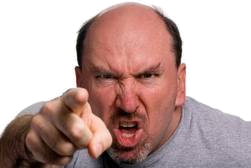
\includegraphics[width=\textwidth]{img/les1-05}
    \vspace*{1cm}
    
\includegraphics[width=\textwidth]{img/les1-06}

  \end{columns}
\end{frame}

\begin{frame}
  \frametitle{The research process}

  \begin{columns}
  \column{\dimexpr\paperwidth}
  \begin{center}
    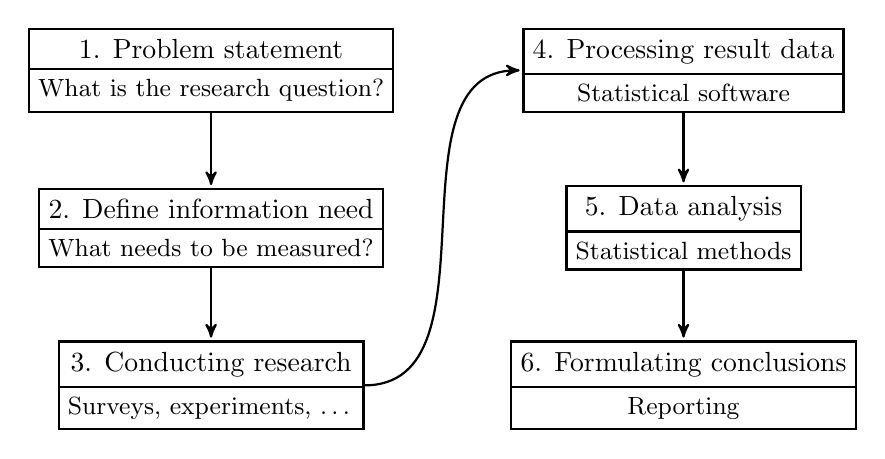
\begin{tikzpicture}[
      auto,
      thick,
      ->,
      >=stealth',
      shorten >=1pt,
      node distance=2cm,
      fase/.style={
        shape=rectangle split,
        rectangle split parts=2,
        ,
        draw}]


      \node[fase] (1) {
        1. Problem statement
        \nodepart{second}
        \small{What is the research question?}
      };
      \uncover<2->{\node[fase] (2) [below of=1] {
        2. Define information need
        \nodepart{second}
        \small{What needs to be measured?}
      };}
      \uncover<3->{\node[fase] (3) [below of=2] {
        3. Conducting research
        \nodepart{second}
        \small{Surveys, experiments, \ldots}
      };}
      \uncover<4->{\node[fase] (4) [right of=1, node distance=6cm] {
        4. Processing result data
        \nodepart{second}
        \small{Statistical software}
      };}
      \uncover<5->{\node[fase] (5) [below of=4] {
        5. Data analysis
        \nodepart{second}
        \small{Statistical methods}
      };}
      \uncover<6->{\node[fase] (6) [below of=5] {
        6. Formulating conclusions
        \nodepart{second}
        \small{Reporting}
      };}

      \uncover<2->{\draw (1) -- (2);}
      \uncover<3->{\draw (2) -- (3);}
      \uncover<4->{\draw (3.east) to [out=0,in=180] (4.west);}
      \uncover<5->{\draw (4) -- (5);}
      \uncover<6->{\draw (5) -- (6);}
    \end{tikzpicture}
  \end{center}
\end{columns}

\end{frame}

\section{Basic concepts in research}

\sectionframelogo{}

\begin{frame}
  \frametitle{Variabeles and values}

  \begin{description}
    \item[Variable] A general property of an object that allows us to distinguish it.
    \item[Value] The specific property of a specific object. The measurement assigned to a variable.
  \end{description}

  \vspace{1cm}

  \begin{columns}[c]
    \column{.6\textwidth}
    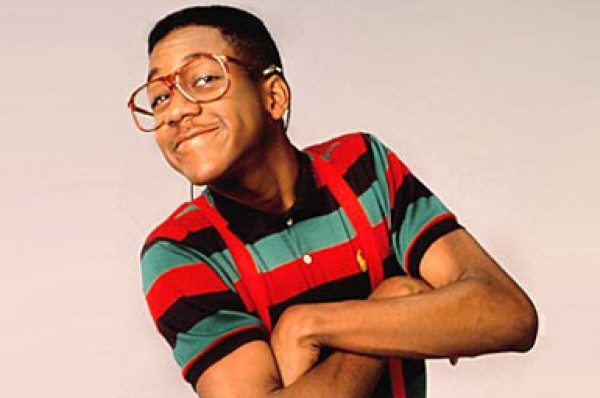
\includegraphics[width=\textwidth]{img/les1-07}

    \column{.4\textwidth}
    \fbox{\parbox{3cm}{%
      \scriptsize
      Variable: gender\\
      Value: male
    }}\\
    \vspace{.5cm}
    \fbox{\parbox{3cm}{%
      \scriptsize
      Variable: height\\
      Value: 180cm
    }}\\
    \vspace{.5cm}
    \fbox{\parbox{3cm}{%
      \scriptsize
      Variable: funny\\
      Value: no
    }}

  \end{columns}
\end{frame}

\begin{frame}
  \frametitle{Levels of measurment}

  Qualitative scales:

  \begin{description}
    \item[Nominal] Categories. E.g. Gender, race, country, \ldots
    \item[Ordinaal] Order. E.g. military rank, level of education \ldots
  \end{description}

\end{frame}

\begin{frame}
  \frametitle{Levels of measurment}

  Quantitative scales:

  \begin{description}
    \item[Interval] Measurement: number + unit, no unique zero value\\
      e.g. 20°C - 15°C = 5°C, but 20°C is \emph{NOT} $1/3$ warmer than 15°C
    \item[Ratio] Measurement w.r.t. absolute zero value. e.g. distance (m), energy (J), mass (kg), \ldots\\
      bv. 20m \emph{is} $1/3$ longer than 15m
  \end{description}
\end{frame}

\begin{frame}
  \frametitle{Relations between variables}

  Variables are related if their values change \emph{systematically}.

  \begin{center}
    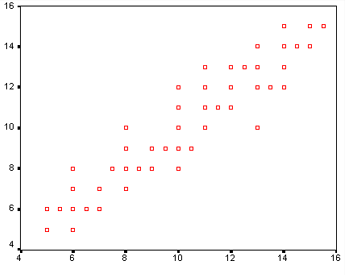
\includegraphics[height=4cm]{img/les1-08a}
    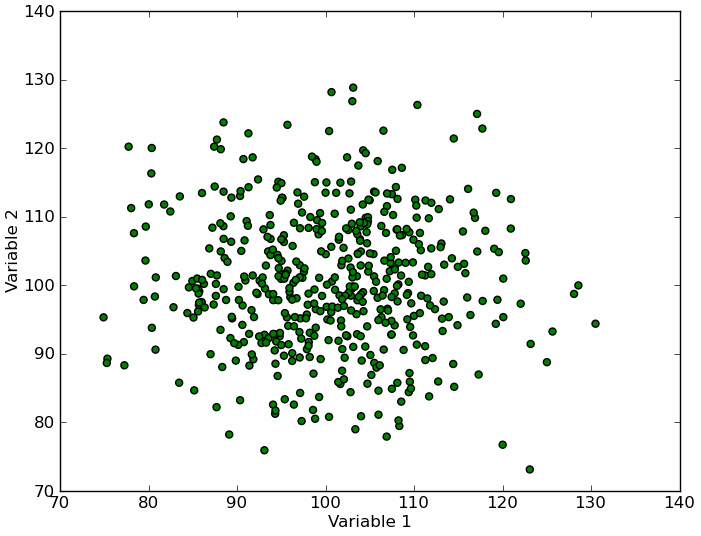
\includegraphics[height=4cm]{img/les1-08b}
  \end{center}
\end{frame}

\begin{frame}
  \frametitle{Relations between variables: example}

  Do people prefer Pepsi or Coca Cola?

  \begin{columns}
    \column{0.99\textwidth}
    \begin{table}
      \centering
      \begin{tabular}{l||c|c||c}
        & Pepsi & Coca Cola & Total \\
        \hline \hline
        Tasty & 56 & 24 & \alert<2>{80} \\
        \hline
        Not tasty & 14 & 6 & \alert<2>{20} \\
        \hline \hline
        Total & \alert<2>{70} & \alert<2>{30} & \alert<2>{100}
      \end{tabular}
    \end{table}

    \only<2>{Marginal totals}

    \column{.01\textwidth}
    \vspace{4cm}
    \hspace*{-2cm}
%    \begin{wrapfigure}{r}{.3\linewidth}
      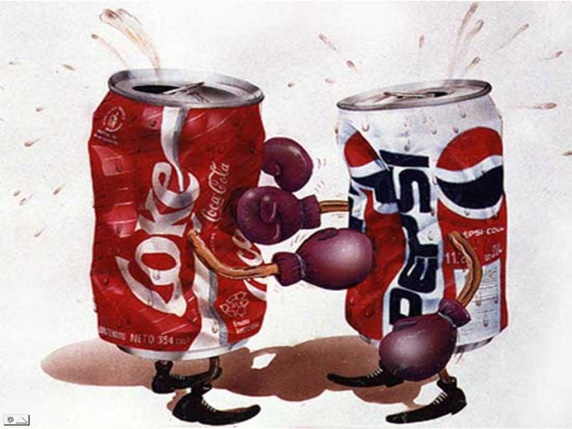
\includegraphics[width=2cm]{img/les1-09}
%    \end{wrapfigure}
  \end{columns}
\end{frame}

\begin{frame}
  \frametitle{Causal relations}

  Researchers are often looking for \textbf{causal relations}, e.g.

  \begin{itemize}
    \item Frustration leads to agression
    \item Alcohol leads to decreased alertness
    \item \ldots
  \end{itemize}

  \begin{description}
    \item[Cause] Independent variable 
    \item[Consequense] Dependent variable
  \end{description}
\end{frame}

\begin{frame}
  \frametitle{Oorzakelijke verbanden}

  \begin{alertblock}{Warning!}
      A relation between variables does not necessarily indicate a \emph{causal} relation!
  \end{alertblock}

  \begin{itemize}
    \item Gaming leads to violent behaviour
    \item Vaccinations cause autism
    \item Correlation between Cola-Light and obesity
    \item \ldots
  \end{itemize}

  \begin{center}
    
\includegraphics[height=2.5cm]{img/les1-10}
  \end{center}
\end{frame}

\end{document}
